%!TEX root = 0卒業論文.tex
\newpage

\section{\rm サイトの説明}
\subsection{画面説明}
制作したサイトでは主にトップページ画面,問題画面,解説画面の3つの画面が存在する.

\subsubsection{トップページ画面}
図\ref{fig:topgamen1}は,本サイトのトップページである.サイトを開いた時,最初に開かれるページである.

\begin{figure}[h]
\begin{center}
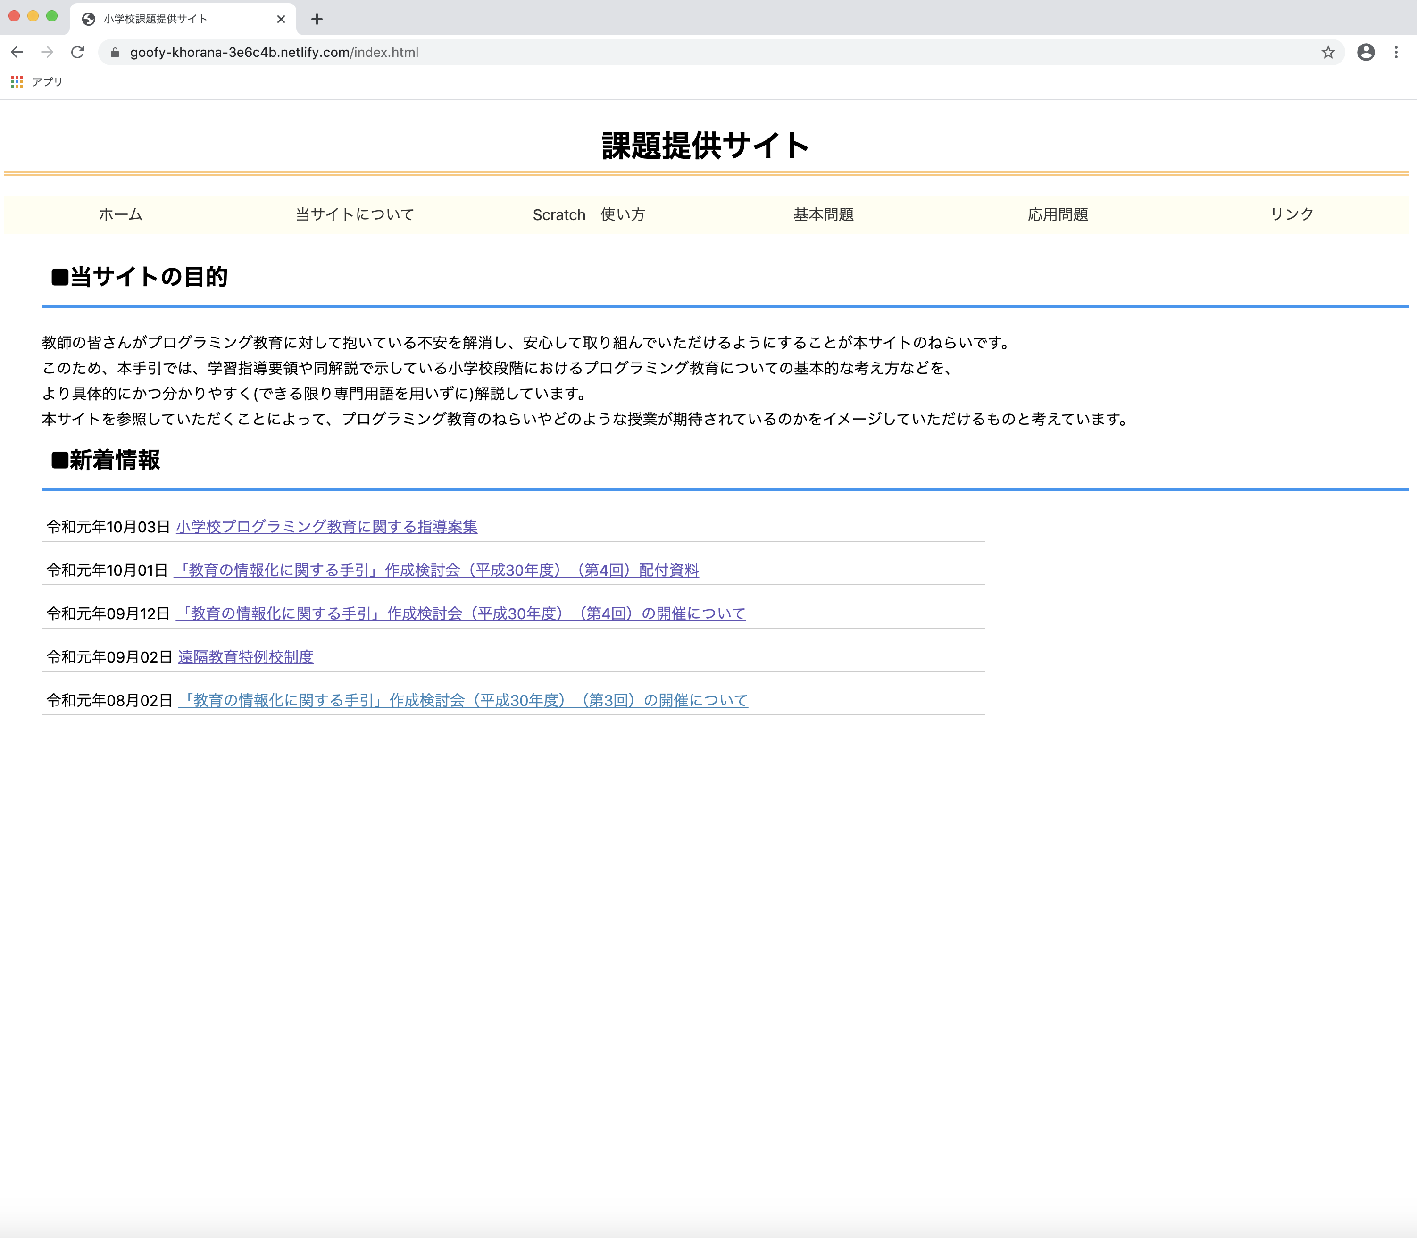
\includegraphics[width=15cm]{toppage.pdf}
\caption{トップページ画面}
\label{fig:topgamen1}
\end{center}
\end{figure}

\newpage
\subsubsection{サイト使用方法画面}
図\ref{fig:tougamen}は,「当サイトについて」である.ここではサイト利用上での注意点を示している.
\begin{figure}[h]
\begin{center}
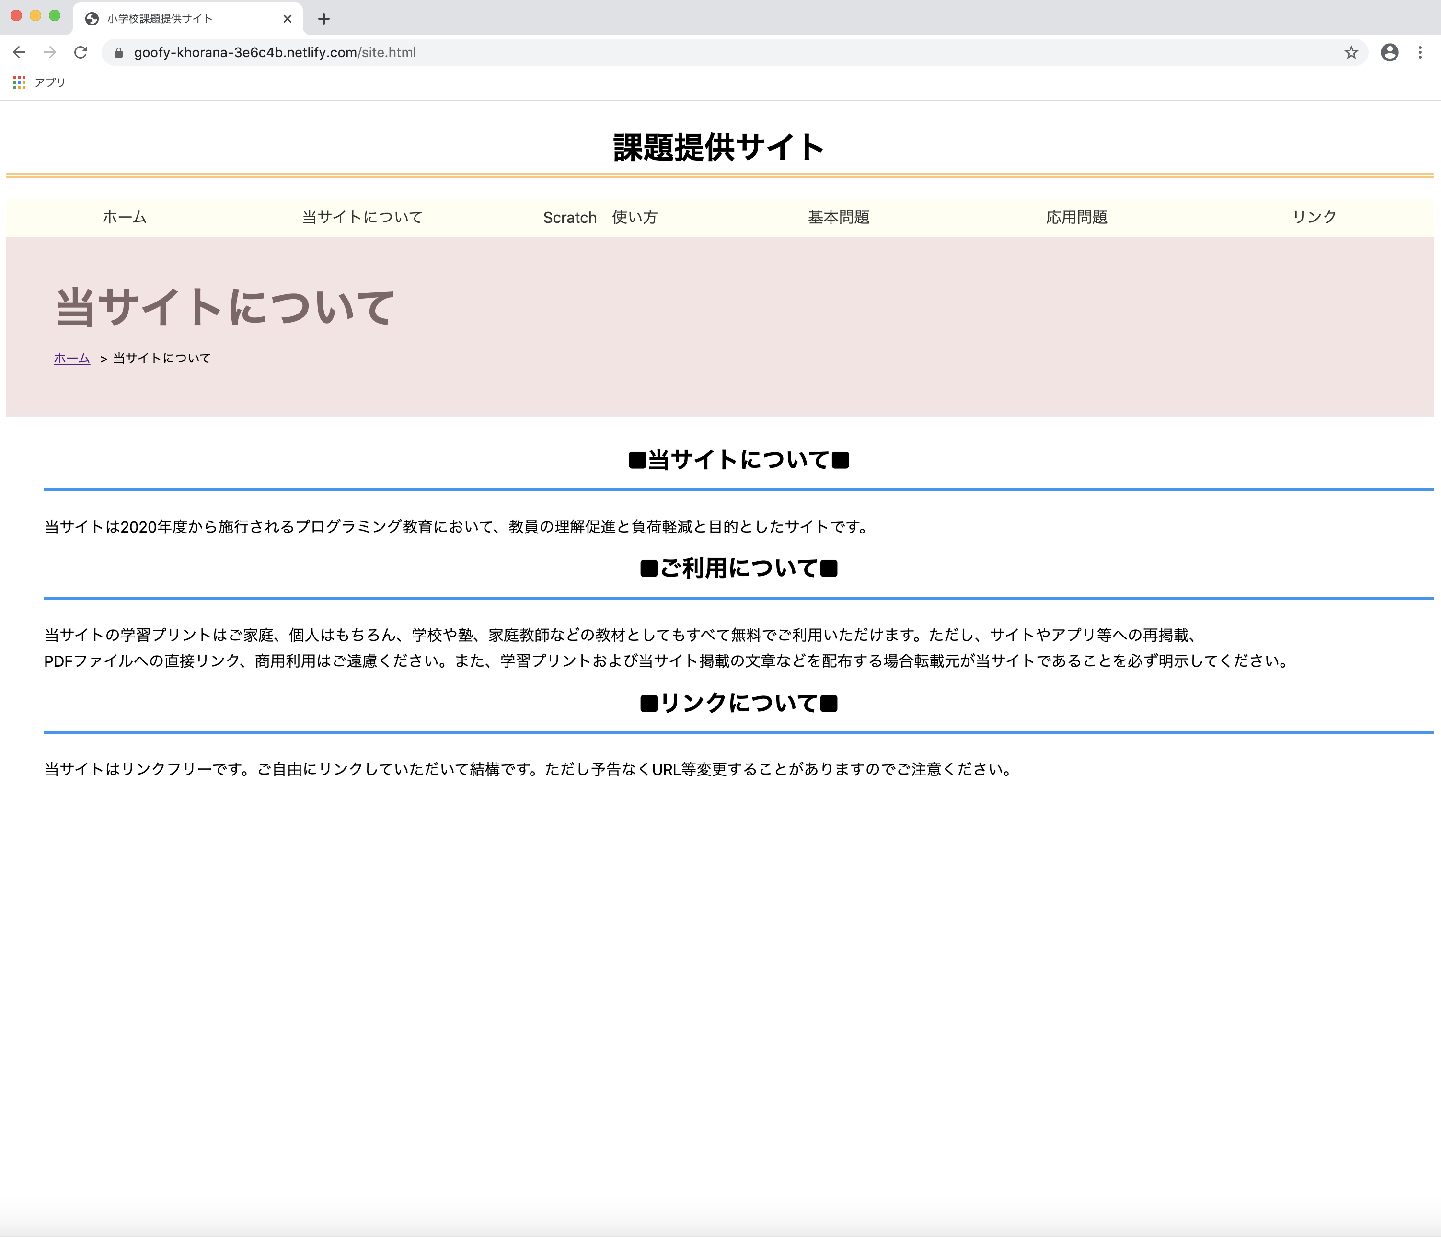
\includegraphics[width=15cm]{site.pdf}
\caption{当サイトについて画面}
\label{fig:tougamen}
\end{center}
\end{figure}

\newpage

\subsubsection{Scrartch使用方法画面}
図\ref{fig:tukaigamen}は,「Scratch使用方法」である.この画面では実際にScratchを使用したことがない方のために,Scratchの使用方法を簡単に説明した画面である.

\begin{figure}[h]
\begin{center}
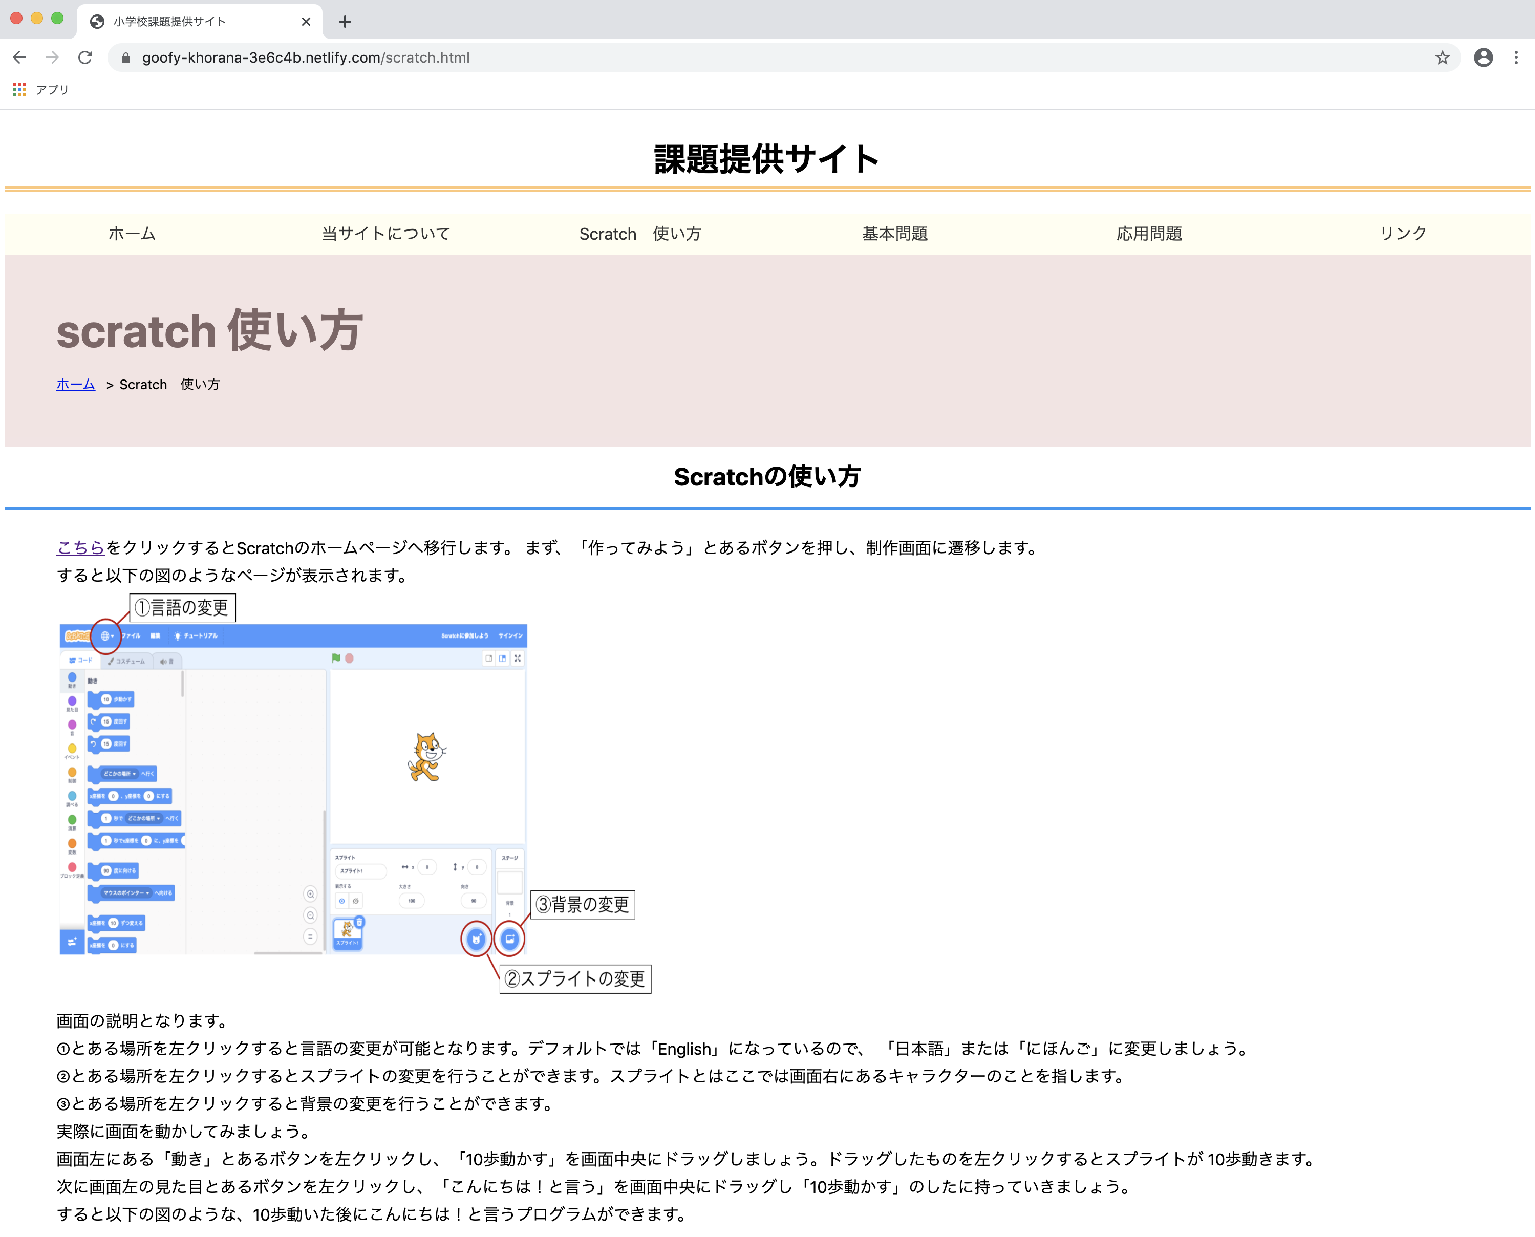
\includegraphics[width=15cm]{Scratch.pdf}
\caption{Scratch 使い方画面}
\label{fig:tukaigamen}
\end{center}
\end{figure}

\newpage

\subsubsection{リンク画面}
図\ref{fig:linkgamen}は,様々なリンクが表示される.文部科学省や学習指導要領など授業で役立つリンクを配置した.

\begin{figure}[h]
\begin{center}
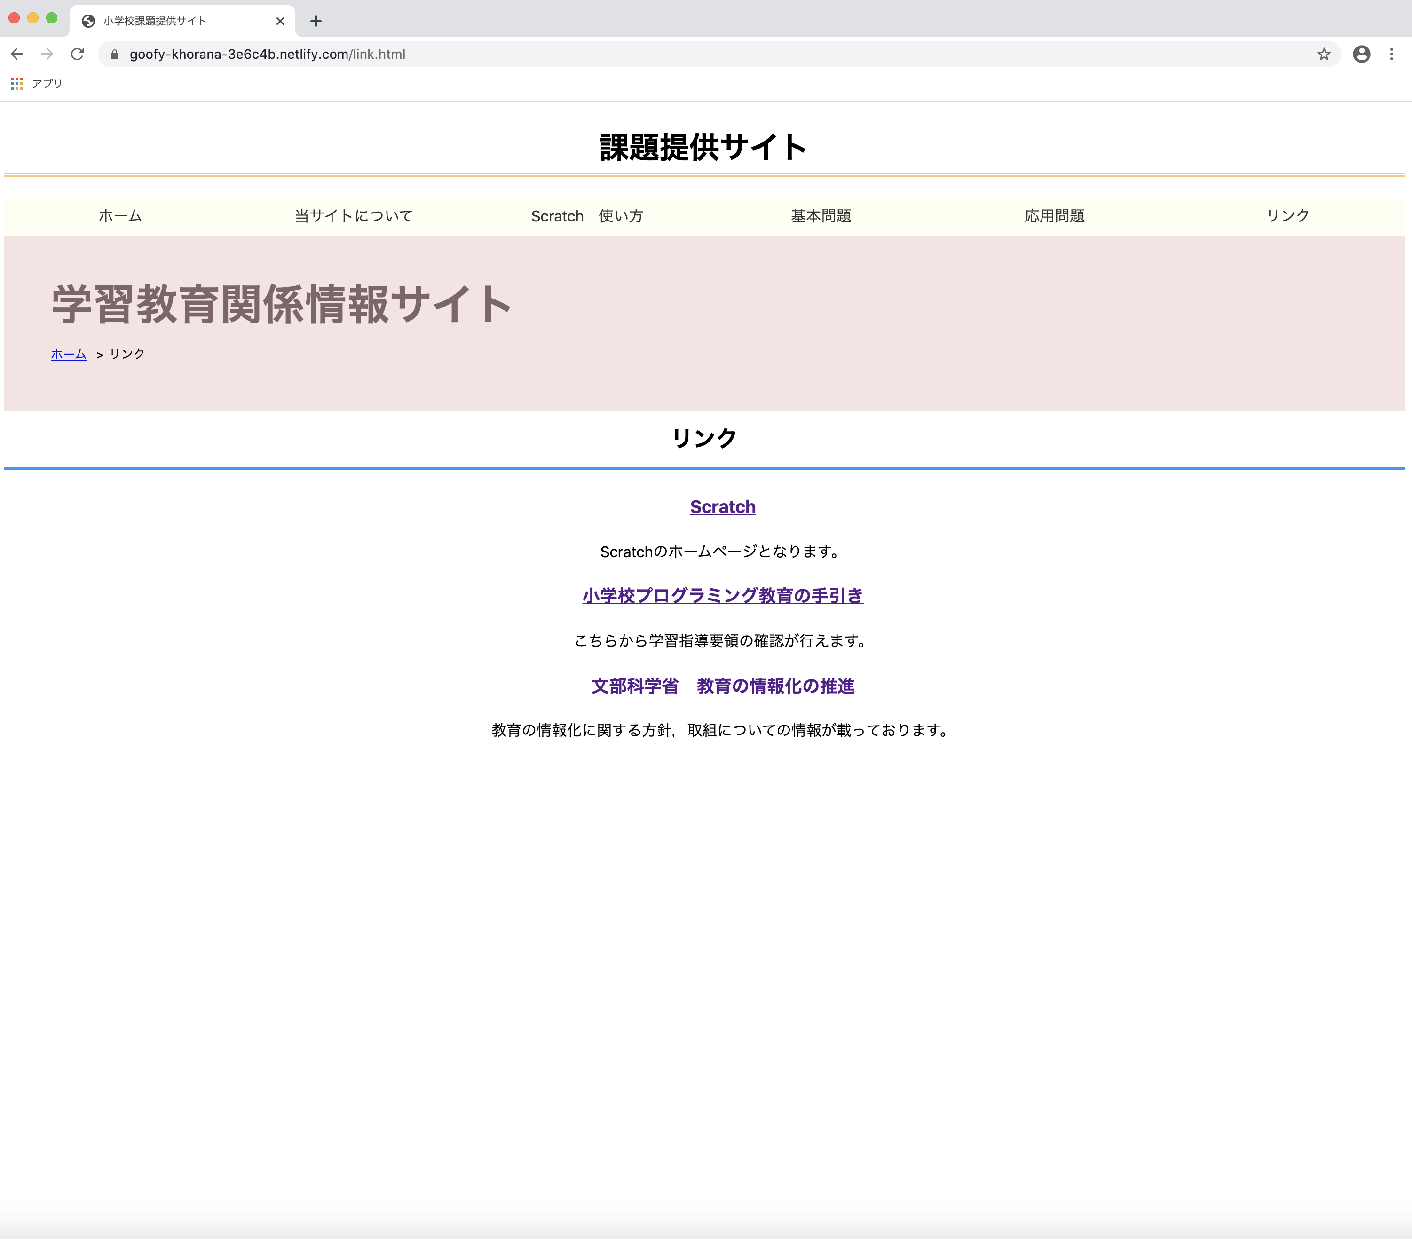
\includegraphics[width=15cm]{Link.pdf}
\caption{リンク画面}
\label{fig:linkgamen}
\end{center}
\end{figure}

\newpage

\subsubsection{問題選択画面}
図\ref{fig:mondaisentaku}は,問題を選択する画面である.ここでは例として順番処理のページを示す.

\begin{figure}[h]
\begin{center}
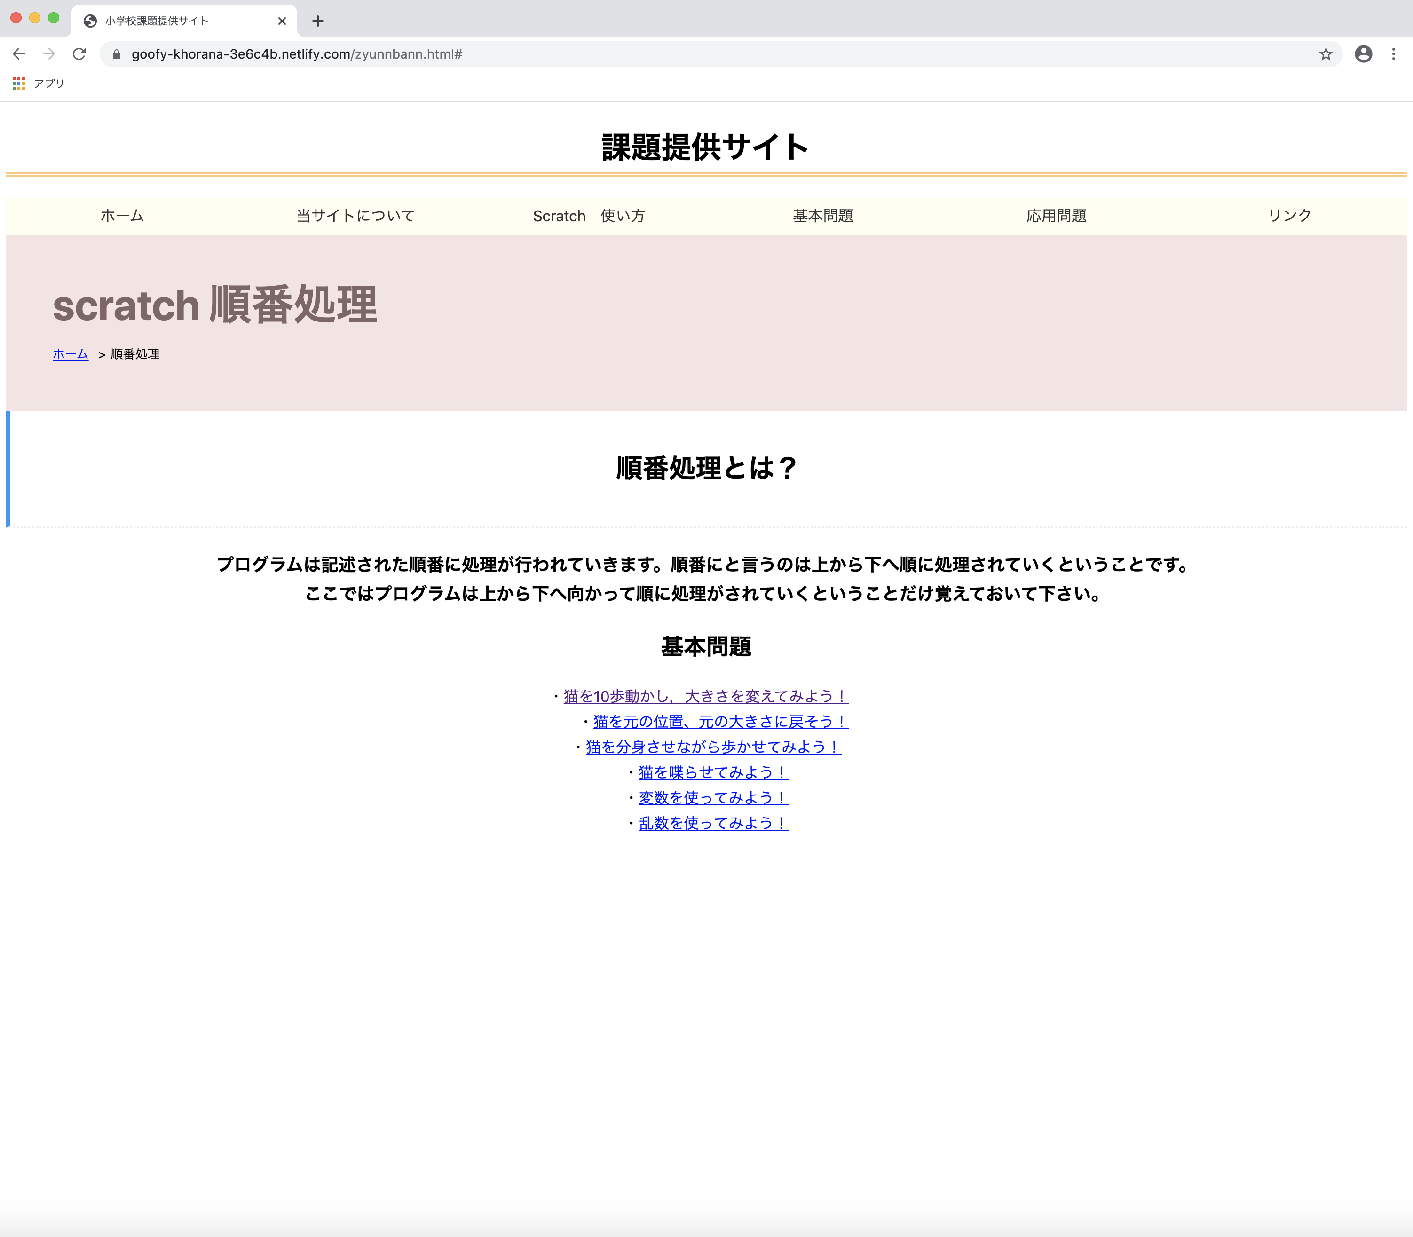
\includegraphics[width=15cm]{zyunnbann.pdf}
\caption{問題選択画面}
\label{fig:mondaisentaku}
\end{center}
\end{figure}

\newpage

\subsection{問題画面}

図\ref{fig:mondaigamen1}は,サイトの問題部分で表示される.この画面で問題が出題される.画面はタイトル部,アニメーション部,ねらい部,ボタン部に分かれている.
各部の説明を表\ref{tab:site1}に示す.
\begin{table}[htb]
\begin{center}
    \caption{問題部画面構成要素説明}
  \begin{tabular}{|c|c|} \hline
     要素名  & 説明  \\ \hline
     タイトル部& 課題のタイトルを部分 \\ \hline
      アニメーション部& 達成すべき目標となるアニメーションを表示する部分 \\ \hline
      ねらい部& 課題を取り組む上でのねらいを表示する部分 \\ \hline
      ボタン部& ホームに戻る,次のページへ,問題の解説を表示する部分\\ \hline
  \end{tabular}
  \label{tab:site1}
  \end{center}
\end{table}
\begin{figure}[h]
\begin{center}
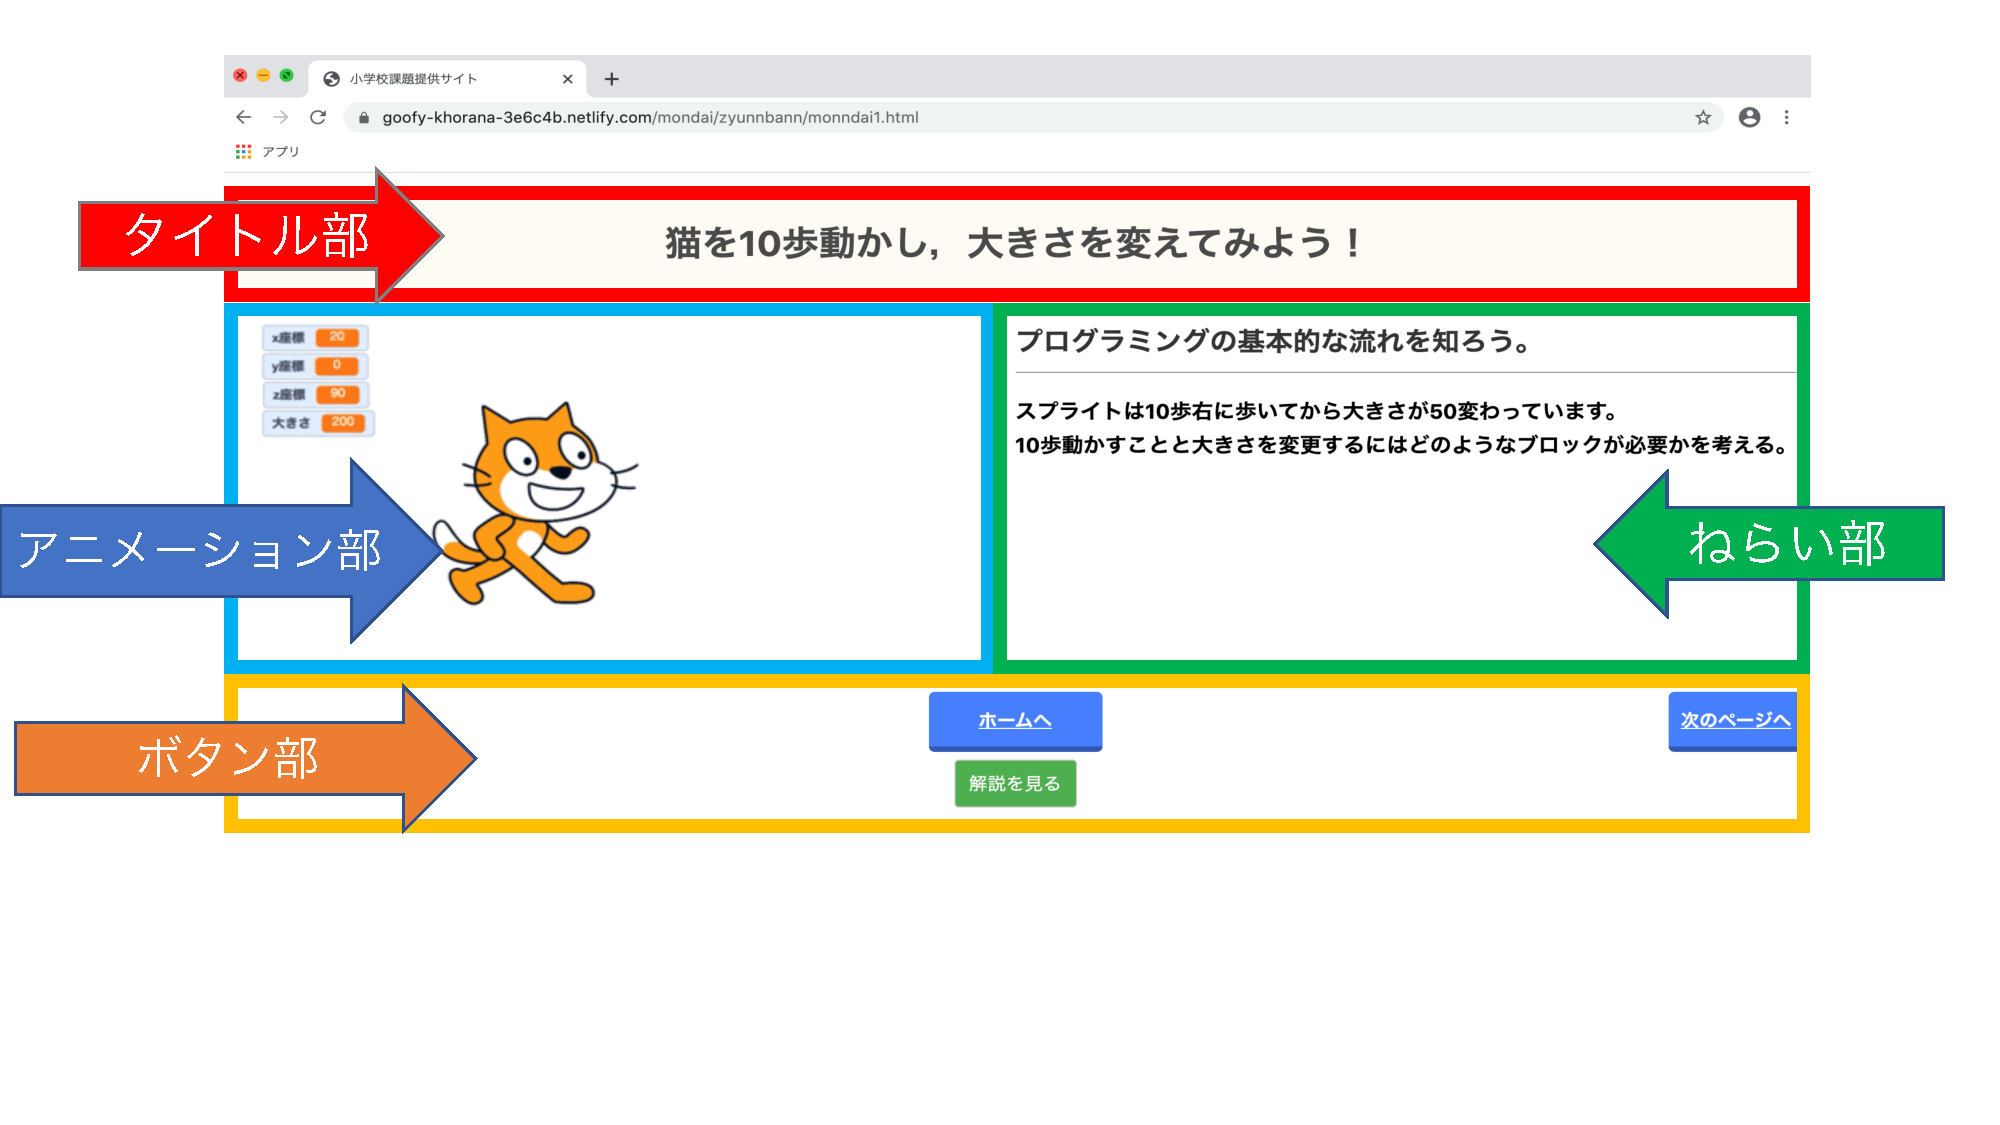
\includegraphics[width=15cm]{mondaigamen.pdf}
\caption{問題画面}
\label{fig:mondaigamen1}
\end{center}
\end{figure}

\newpage

\subsection{解説画面}
図\ref{fig:zyunnbannkaisetu}は,問題画面の「解説を見る」ボタンを押すことで表示される.
\begin{figure}[h]
\begin{center}
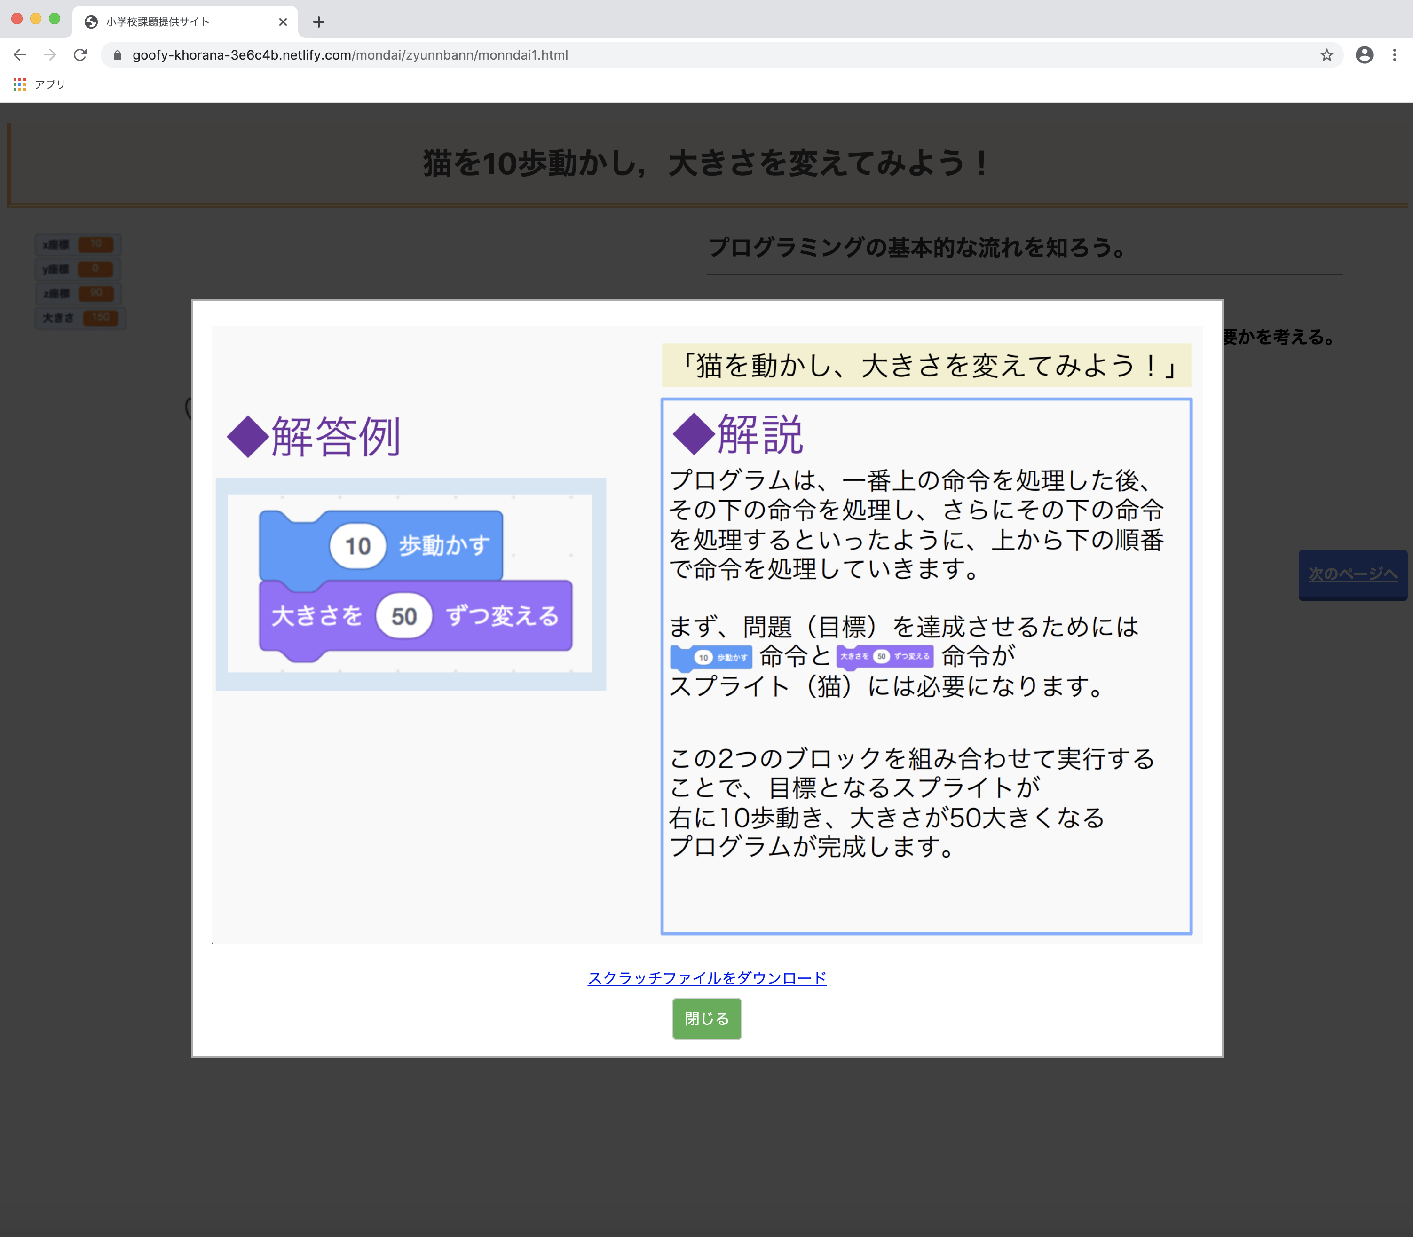
\includegraphics[width=15cm]{zyunnbannkotae.pdf}
\caption{解説画面}
\label{fig:zyunnbannkaisetu}
\end{center}
\end{figure}

\newpage


\subsection{操作説明}
サイトの操作説明を行う.トップページ画面,問題画面,解説画面はページ遷移ボタンのみである.
\subsubsection{問題画面の流れ}
\begin{enumerate}
 \item 課題のテーマが問題画面上部に表示される
 \item 出された課題を達成するため,課題のアニメーション,課題のねらいを読み,取り組む.
 \item 「解説を見る」を押し,解説とスクラッチファイルを用いて課題を理解する.
 \item 理解できたのであれば,「次のページへ」ボタンで画面遷移する. 
\end{enumerate}

















